\chapter{Sources of data}

\section{Data volunteered by users}
Established conduits: app store reviews, in-app feedback integration (mobile twin peaks), structured emails (c.f. Android Daisy Reader and Kiwix Android for examples).
\begin{itemize}
    \item Social Media channels:
    \item Structured emails:
\end{itemize}

Android Daisy Reader example:

Kiwix-Android example and screenshots:

\url{https://github.com/kiwix/kiwix-android/issues/335}

\url{https://github.com/kiwix/kiwix-android/pull/351/files}

Brief discussion on the benefits of users volunteering and providing feedback. `Conversations' in Android Reviews. Limitations.

\section{Alpha, Beta, and similar testing}
Add some examples and limitations from Android and Google Play.

\section{Code Quality}
Static Analysis, that assesses the source code, the resources, and the generated files (including the APK file for Android apps). 

Tracking Android app metrics (method count (e.g. using tools such as dexcount \url{https://github.com/KeepSafe/dexcount-gradle-plugin}, size of the binary) \url{https://medium.com/@emmaguy/tracking-android-app-metrics-431cbea2113d}

% Tools to consider include danger.systems and stathat (both mentioned in Emma Guy's article) http://www.stathat.com/manual/start (co-developed by the CTO of OkCupid)

\section{Google Play Console}
\subsection{Android Vitals}


\begin{figure}[htbp]\centering
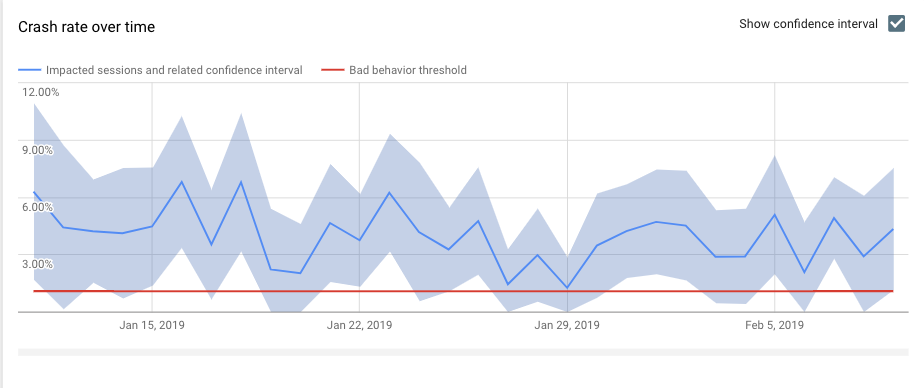
\includegraphics[width=0.5\textwidth]{images/Crash-rate-graph-for-kiwix-with-confidence-interval.png}
\caption{30-day Crash rate for Kiwix.}
\label{crashrate}
\end{figure}


\begin{table}[htbp]
\caption{Crashes of Kiwix by Android Version}

\begin{center}
\begin{tabularx}{\columnwidth}{|X|X|X|X|X|}
\hline
\textbf{Version} & \textbf{\textit{Impacted sessions}}& \textbf{\textit{Crash-free sessions}}& \textbf{\textit{\#Sessions}} & \textbf{\textit{Bottom quartile}} \\
\hline
9& 8.28\%& 91.72\%&~3k&1.70\%  \\
\hline
8.1.0&7.39\%&92.61\%&~6k&1.29\% \\
\hline
8.0.0&4.89\%&95.11\%&~13k&1.19\% \\
\hline
7.0&2.08\%&97.92\%&~4k&0.75\% \\
\hline
6.0.1&1.40\%&98.60\%&~3k&0.75\% \\
\hline
\end{tabularx}
\label{tab1}
\end{center}
\end{table}

\subsection{Ratings and Reviews}
\subsection{Release Management}

\section{Application-generated data}
\begin{itemize}
    \item Logging: Android log, remote logging (log shipping, etc.)
    \item Mobile Analytics client libraries
\end{itemize}

\subsection{Improving the value and utility of the data}

Operability (O11y), wrap calls in web server to record time taken\url{https://www.honeycomb.io/blog/tell-me-more-nginx/}, (via \url{https://twitter.com/mipsytipsy/status/1124933206585769991})

Structured Logging \texttt{ label=value }.

\section{Heatmaps and other GUI tracking methods}


\section{Experiences using Android Vitals}
To be continued... Base on my paper \textit{"Google Play Console: Insightful Development using Android Vitals and Pre-Launch Reports"}  \url{https://www.overleaf.com/project/5c61b2d5691bcf6ed5f653e5} and more recent work for the Kiwix family of applications, see  \textit{"Symbiosis between Google Play Console and Testing Android Apps"} \url{https://www.overleaf.com/project/5c921d72bd9930036341e61d}.

\hypertarget{dynamiclogging}{\section{Dynamic Distributed Logging and Analytics}}
To be continued... Base on my draft paper titled \textit{Dynamic Distributed Logging and Analytics} \url{https://www.overleaf.com/project/5c9786c40258920bedac0e18}. Explain the rationale (privacy, performance, efficacy). Discuss design and implementation aspects, data ownership, data transmission using mobile connectivity (price, availability, opportunity cost of sending this rather than content for the user, etc.)

\subsection{Datensparsamkeit}
\textit{The following is a repeat from my notes in the introduction. I've added it here since this is where I'm going to develop the concepts and ideas.}

 There are also ethical and other concerns related to collecting and keeping data, concepts such as Datensparsamkeit\cite{fowler_datensparsamkeit_2013} (data minimisation) apply. Furthermore, investigating the relationship between the amount of data and its value and utility may help both researchers and practitioners. And establishing dynamic heuristics to govern what data to collect, transmit, and utilise may also reduce any data burden (the burden of collecting, transmitting, processing, safe-keeping, and storing data).
 
 \subsection{Effects of decomposing data}
 Logging Before and After can help us to reproduce a similar transition as part of our testing, for instance where a user changed the interface language from English to Hindi. However, perhaps logging and transmitting the before and after may intrude on their privacy and be contrary to Datensparsamkeit? Would recording that they changed the interface language be sufficient? Conversely, perhaps collecting additional information would be valuable such as the Wikipedia content they are currently accessing? (since there may be bugs in how the content is being presented that the user tried to address by changing the interface language).
 
 \section{Material gaps in existing data}
 \textit{See also the section on dissonance, etc.}
 
 \section{Designing and implementing Mobile Analytics}
 \url{https://medium.com/wantedly-engineering/better-analytics-in-android-with-annotation-processing-and-kotlinpoet-bffca3f24c37}